
\section{Results}
\label{sec:results}

The data and SM predictions are shown for all events in 
Fig.~\ref{fig:pfmet_eemm}, 
and split between the $ee$
and $\mu\mu$ final states in 
Fig.~\ref{fig:pfmet_ee} and \ref{fig:pfmet_mm}. 
We observe 14 events (7 in each lepton flavor channel) 
%We observe 7  events (all in the $\mu\mu$ channel) %2010
in the loose signal region (MET $>$ \signalmetl GeV), 
compared to a data-driven prediction of 
13.6 $\pm$ 1.14,
%$6.0 \pm 0.8$, %2010
which is dominated by the estimated \ttbar contribution. 
For the tight signal region defined by MET $>$ \signalmett GeV, 
we observe 2 events (both in the $\mu\mu$ channel) compared to a 
data-driven prediction of 
1.32 $\pm$ 0.34.
%$1.2 \pm 0.4$. %2010
These uncertainties are statistical only, and systematic uncertainties will be 
discussed in Sec.~\ref{sec:systematics}. We conclude that no excess of signal 
with respect to the data-driven prediciton is observed.

%When we have enough data, we will display in the figures the predicted $t\bar{t}$ MET distribution obtained by scaling the $e\mu$ distribution
%in data. However, due to limited statistics we cannot currently do this. Therefore 
For display purposes only, we have taken the
$t\bar{t}$ MET distribution from MC and normalized it such that the integral for 
MET$>$\signalmetl~GeV matches the data-driven prediction
from the OF subtraction. 
%{\bf I don't know if we want to do this in the final plots.} It's probably fine.

%We observe a slight excess of observed
%MET with respect to the data driven prediction in the bulk of the distribution. Systematic effects which may contribute
%to this excess, including lepton mismeasurement and effects related to pile up, will be assessed in Sec.~\ref{sec:systematics}.


\newcommand{\resultcaption}[1]{
      The observed MET distribution for data in the #1 channels (black points),
      predicted $t\bar{t}$ MET distribution (red line), the sum of predicted 
	  $t\bar{t}$ MET distribution and
      Z  MET  distribution  predicted  from photon  MET  templates
      (solid blue line),  and MC stacked for dominant backgrounds. 
	  %Here $VV$  indicates the sum
      %of  $WW$,  $WZ$  and  $ZZ$, while  additional  backgrounds  from
      %$W+$jets   and   single  top   are   omitted   since  they   are
      %negligible.  
	  Below the  plot is  tabulated the  integral  of the
      predicted  MET distribution  using the  MET templates  method (Z
      pred),  the  predicted ttbar  yield  using  the opposite  flavor
      subtraction  technique (OFOS), the  sum of  these two
      contributions (Z pred + OFOS), and the observed MET distribution
      (data), for MET $>$ 30~GeV and $>$ 60~GeV (which are shown as cross
	  checks), and for the signal regions of MET $>$ 100~GeV and $>$ 200~GeV. 
	  %TO ADD
	  %The quantity pull  = (data-Z prediction)/(Z prediction)  is shown on
      %top of the  plot.  
}

\begin{figure}[hbtp]
  \begin{center}
    \resizebox{1.0\linewidth}{!}{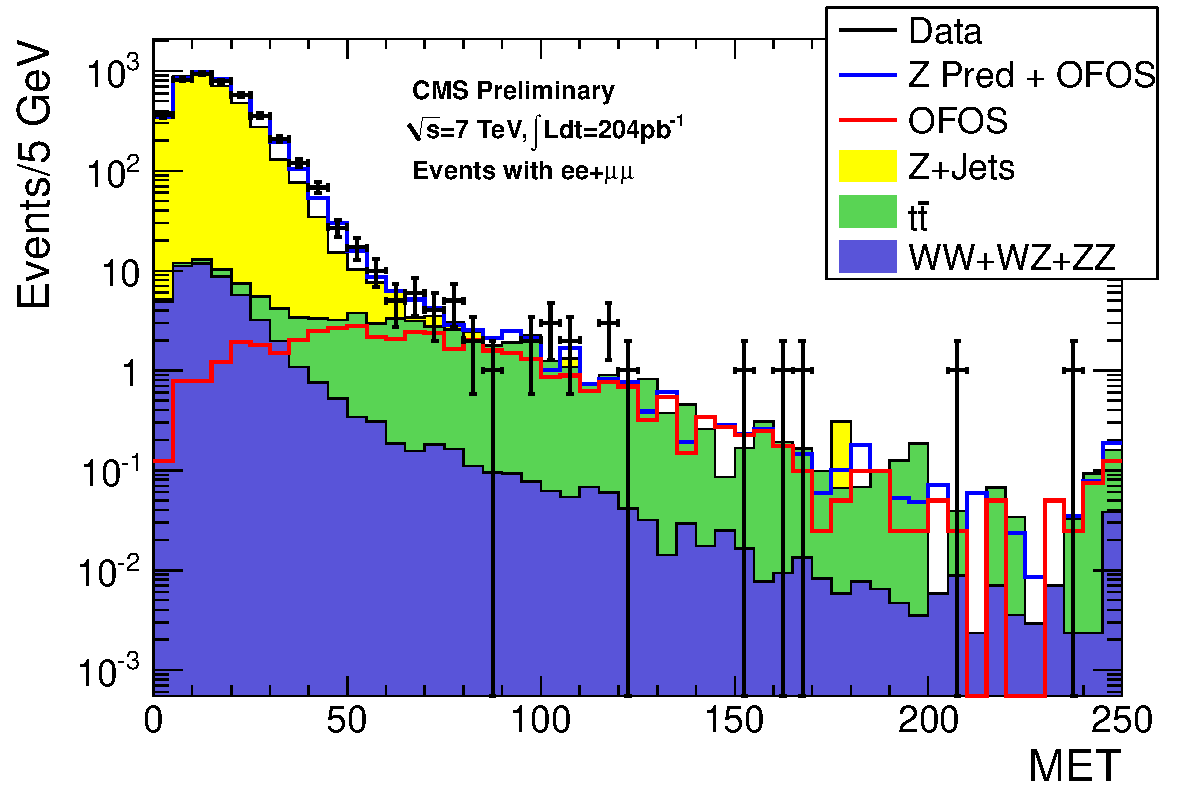
\includegraphics{plots/lep_metPredicted.pdf}}

	\medskip 

    %\resizebox{\linewidth}{!}{
    \begin{tabular}{lcccc}
\hline
                        &   N(MET $>30$)  GeV    &   N(MET $>60$)  GeV    &   N(MET $>100$) GeV    &   N(MET $>200$) GeV \\
\hline
        Z pred  &  406.54  $\pm$  6.82  &   14.63  $\pm$  1.27  &    1.82  $\pm$  0.60  &    0.19  $\pm$  0.07 \\
          OFOS  &   54.77  $\pm$  2.09  &   34.73  $\pm$  1.67  &   11.76  $\pm$  0.97  &    1.13  $\pm$  0.33 \\
\hline
 Z pred + OFOS  &  461.31  $\pm$  7.13  &   49.36  $\pm$  2.10  &   13.59  $\pm$  1.14  &    1.32  $\pm$  0.34 \\
\hline
          Data  &                  488  &                   39  &                   14  &                    2 \\


%2010
%              Z pred    &  38.47  $\pm$  0.90    &   1.81  $\pm$  0.13    &   0.14  $\pm$  0.03   \\
%                OFOS    &   6.43  $\pm$  1.00    &   4.24  $\pm$  0.82    &   1.10  $\pm$  0.42   \\
%\hline
%       Z pred + OFOS    &  44.90  $\pm$  1.35    &   6.04  $\pm$  0.82    &   1.24  $\pm$  0.42   \\
%\hline
%                data    &                  51    &                   7    &                   0   \\
\hline
    \end{tabular}

    \caption{ \resultcaption{$ee$ and $\mu\mu$} }
    \label{fig:pfmet_eemm}
  \end{center}
\end{figure}

\begin{figure}[hbtp]
  \begin{center}
    \resizebox{1.0\linewidth}{!}{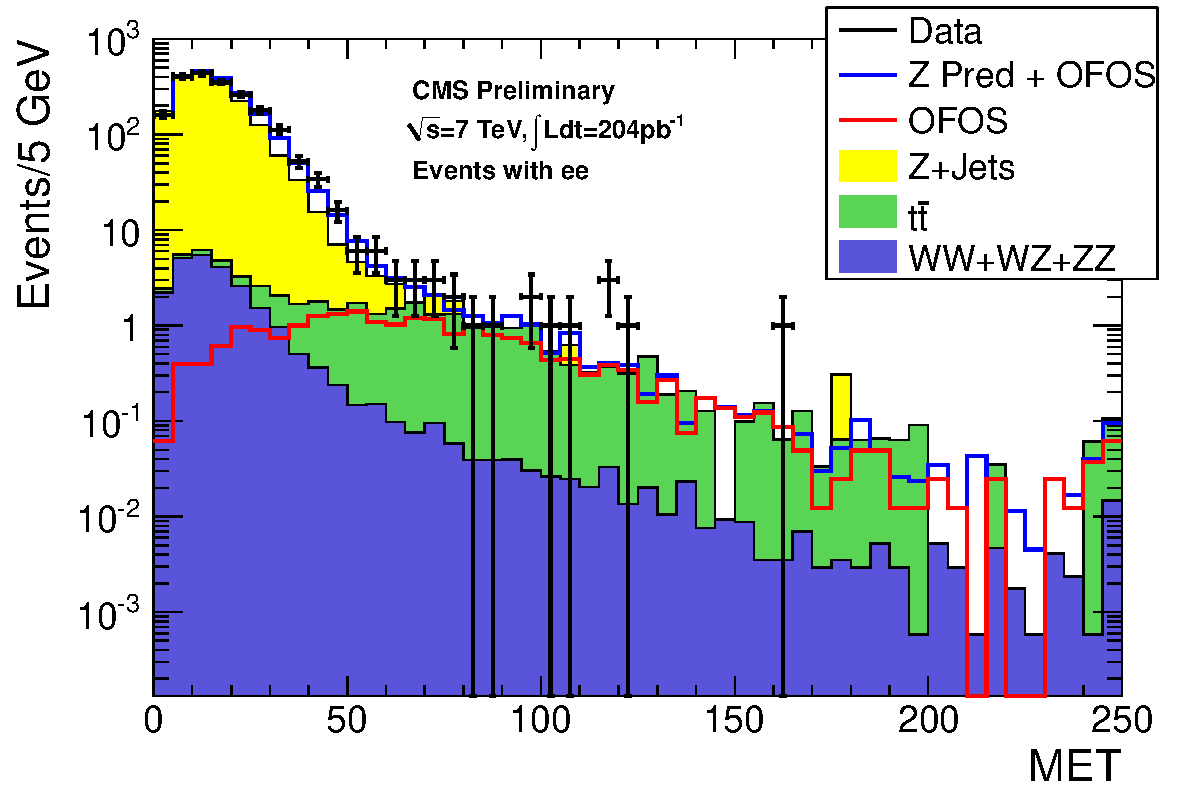
\includegraphics{plots/lep_metPredicted_ee.pdf}}

	\medskip 

    %\resizebox{\linewidth}{!}{
    \begin{tabular}{lcccc}
\hline

                        &   N(MET $>30$)  GeV    &   N(MET $>60$)  GeV    &   N(MET $>100$) GeV    &   N(MET $>200$) GeV \\
\hline
        Z pred  &  195.06  $\pm$  3.25  &    7.35  $\pm$  0.63  &    0.94  $\pm$  0.30  &    0.11  $\pm$  0.05 \\
          OFOS  &   25.60  $\pm$  1.38  &   16.24  $\pm$  1.10  &    5.50  $\pm$  0.64  &    0.53  $\pm$  0.22 \\
\hline
 Z pred + OFOS  &  220.66  $\pm$  3.53  &   23.59  $\pm$  1.27  &    6.44  $\pm$  0.71  &    0.64  $\pm$  0.22 \\
\hline
          Data  &                  249  &                   22  &                    7  &                    0 \\


%2010
%                        &   N(MET $>30$)  GeV    &   N(MET $>60$)  GeV    &   N(MET $>120$) GeV   \\
%\hline
%              Z pred    &  16.45  $\pm$  0.37    &   0.79  $\pm$  0.05    &   0.06  $\pm$  0.01   \\
%                OFOS    &   2.88  $\pm$  0.45    &   1.90  $\pm$  0.36    &   0.49  $\pm$  0.19   \\
%\hline
%       Z pred + OFOS    &  19.32  $\pm$  0.58    &   2.68  $\pm$  0.37    &   0.56  $\pm$  0.19   \\
%\hline
%                data    &                  22    &                   0    &                   0   \\
\hline
    \end{tabular}

    \caption{ \resultcaption{$ee$} }
    \label{fig:pfmet_ee}
  \end{center}
\end{figure}

\begin{figure}[hbtp]
  \begin{center}
    \resizebox{1.0\linewidth}{!}{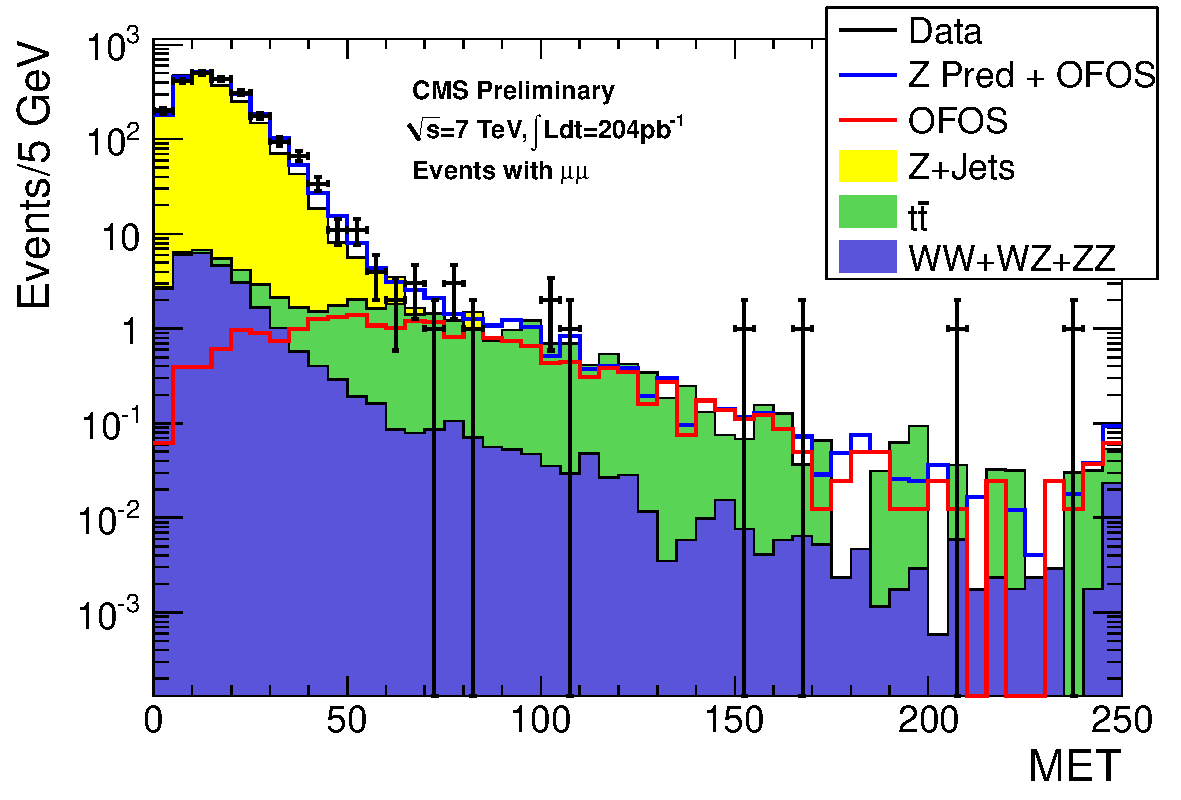
\includegraphics{plots/lep_metPredicted_mm.pdf}}

	\medskip 

    %\resizebox{\linewidth}{!}{
    \begin{tabular}{lcccc}
\hline
                        &   N(MET $>30$)  GeV    &   N(MET $>60$)  GeV    &   N(MET $>100$) GeV    &   N(MET $>200$) GeV \\
\hline
        Z pred  &  211.48  $\pm$  3.60  &    7.28  $\pm$  0.65  &    0.88  $\pm$  0.31  &    0.08  $\pm$  0.03 \\
          OFOS  &   29.16  $\pm$  1.57  &   18.49  $\pm$  1.25  &    6.26  $\pm$  0.73  &    0.60  $\pm$  0.25 \\
\hline
 Z pred + OFOS  &  240.64  $\pm$  3.93  &   25.77  $\pm$  1.41  &    7.15  $\pm$  0.79  &    0.68  $\pm$  0.25 \\
\hline
          Data  &                  239  &                   17  &                    7  &                    2 \\

%2010
%                        &   N(MET $>30$)  GeV    &   N(MET $>60$)  GeV    &   N(MET $>120$) GeV   \\
%\hline
%              Z pred    &  22.03  $\pm$  0.54    &   1.02  $\pm$  0.08    &   0.08  $\pm$  0.02   \\
%                OFOS    &   3.55  $\pm$  0.55    &   2.34  $\pm$  0.45    &   0.61  $\pm$  0.23   \\
%\hline
%       Z pred + OFOS    &  25.58  $\pm$  0.77    &   3.36  $\pm$  0.46    &   0.68  $\pm$  0.23   \\
%\hline
%                data    &                  29    &                   7    &                   0   \\
\hline
    \end{tabular}

    \caption{ \resultcaption{$\mu\mu$} }
    \label{fig:pfmet_mm}
  \end{center}
\end{figure}


